% !TEX root = owasp-doc.tex

% ================================================
%	OVERVIEW
% ================================================

\headerimage
\chapter{Overview}

\section{Who is This For?}
This checklist is for technology and business leadership in an organization
to consider all aspects and tasks needed to map out a Large Language Model
strategy.

Recent advances in artificial intelligence (AI) have emphasized the importance
of organizations developing a plan to maintain proper relationship balance
with AI.

\begin{itemize}
  \item \textbf{Artificial intelligence} (AI) is a broad term that encompasses
  all fields of computer science that enable machines to accomplish tasks that
  would normally require human intelligence. Machine learning and generative AI
  are two subcategories of AI.
  \item \textbf{Machine learning} is a subset of AI that focuses on creating
  algorithms that can learn from data. Machine learning algorithms are trained
  on a set of data, and then they can use that data to make predictions or
  decisions about new data.
  \item \textbf{Generative AI} is a type of machine learning that focuses on
  creating new data.
\end{itemize}

\begin{figure}[h]
  \centering
  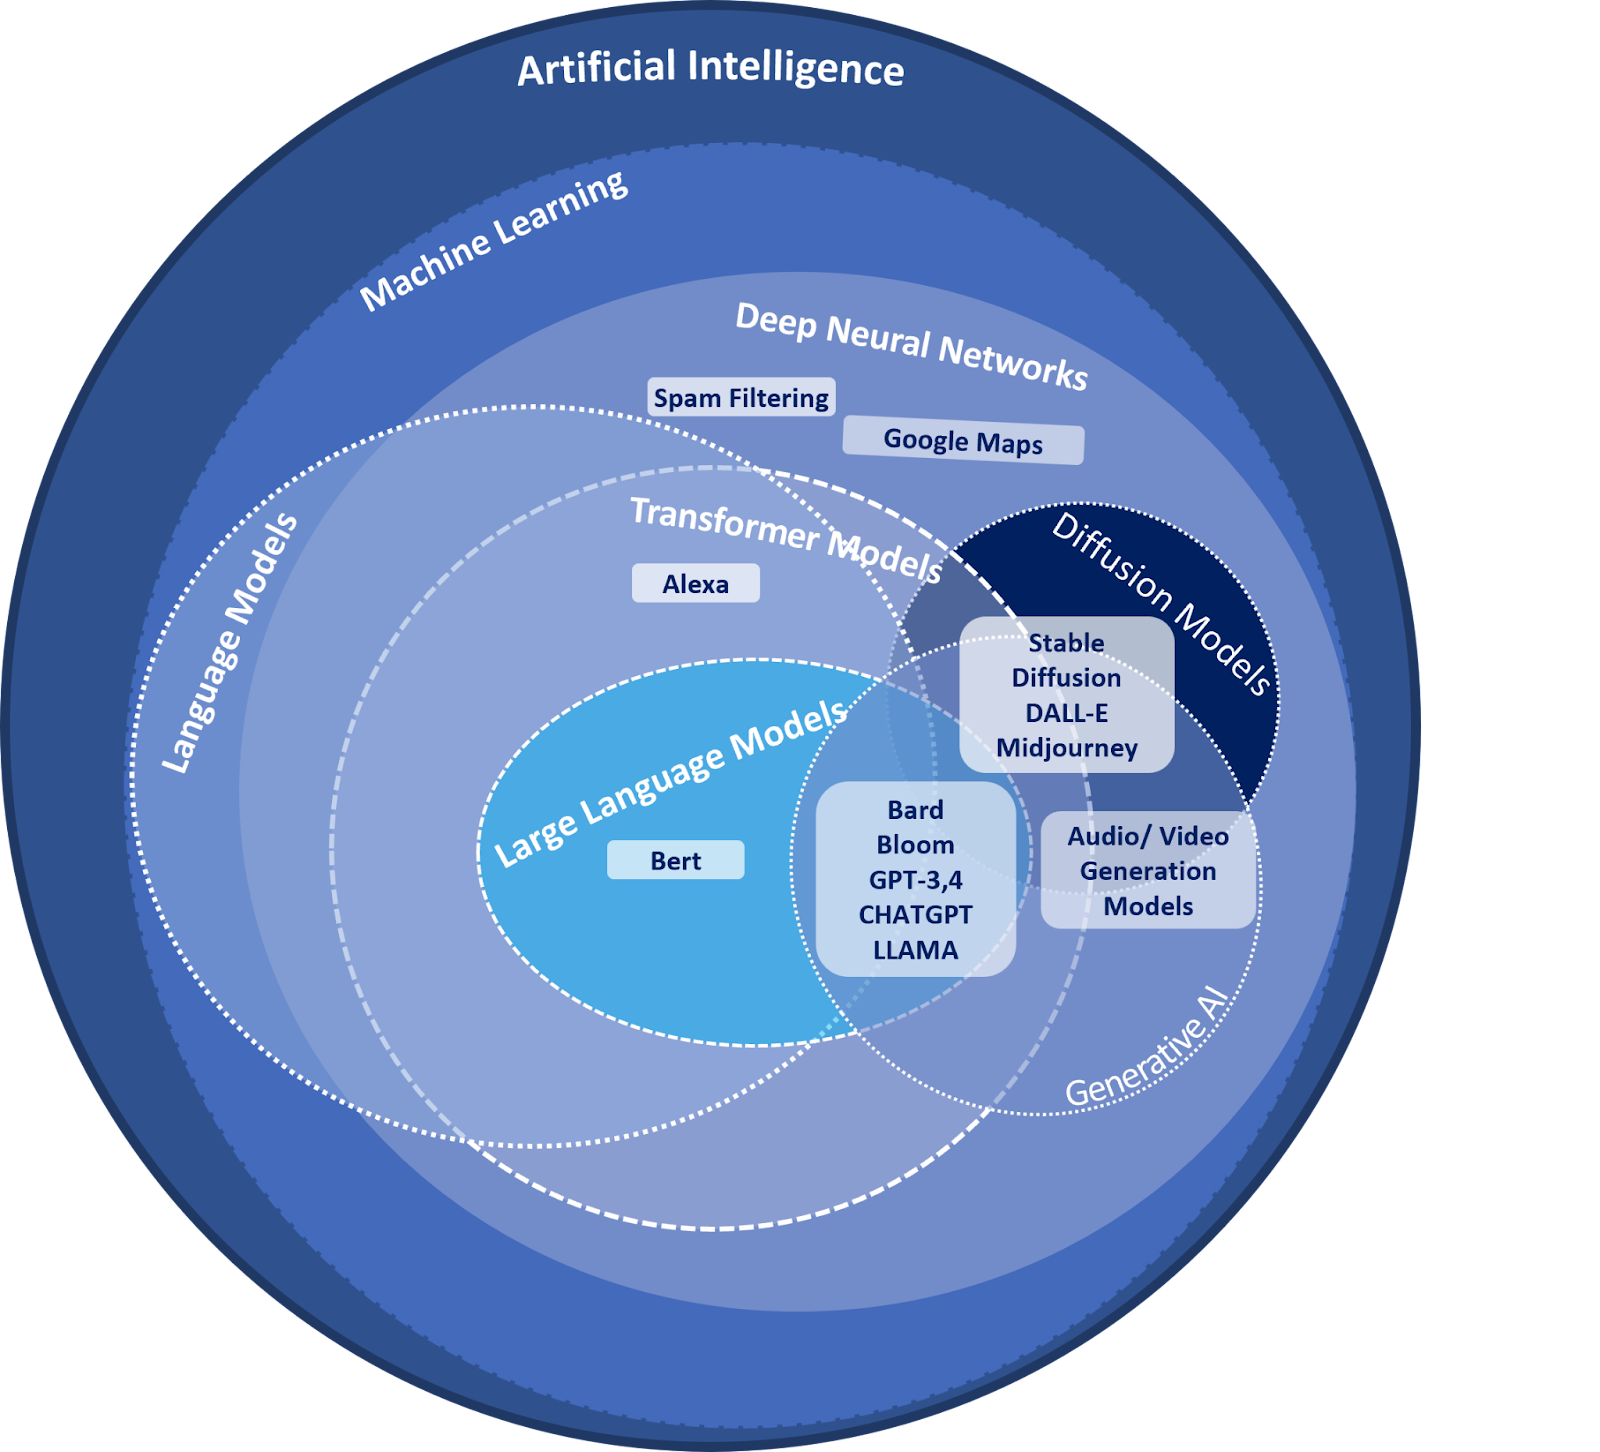
\includegraphics[width=\textwidth]{ai_llm_relationship}
  \caption{Image of LLM relationship within the field of Artificial Intelligence}
  \label{fig:ai-llm-relationship}
\end{figure}

\section{How to Use This Document}

For decades, researchers have been working on artificial intelligence, large
language models, and diffusion models. Still, new improvements in training data
availability, computer power, GenAI capacity, and the release of solutions like
ChatGPT, ElevenLabs, and Midjourney have made the field more popular and led to
its growth. Every internet user and business should prepare itself for the
impact of a surge in powerful GenAI applications. GenAI holds enormous promise
and opportunities for discovery, efficiency, and driving corporate growth across
many industries and disciplines. However, as with any strong new technology, it
introduces new challenges to security and privacy.

Executive, technology, cybersecurity, privacy, compliance, and legal leaders
must pay close attention to the fast GenAI technological transformation and
devise a strategy to benefit from opportunities while fighting against threats
and managing risks.

Organizations will face challenges in controlling users who want to use these
technologies against them, as well as business leaders who see potential to
employ them to better their organization.

Many applications within a business employ artificial intelligence
applications, such as human resource hiring, SPAM detection for email,
behavioral analytics for SIEM, and MDR apps. The primary focus of this document
is on Large Language Model applications, which can produce content.

\clearpage

\section{Responsible and Trustworthy Artificial Intelligence}

As challenges and benefits of Artificial Intelligence emerge and regulations and
laws are passed, the principles and pillars of responsible and trustworthy is
evolving from ideal objects and concerns to future established standards. The
OWASP AI Security and Privacy Guide working group is monitoring these changes
and addressing the larger and more difficult considerations for all aspects of
artificial intelligence.

\begin{figure}[h]
  \centering
  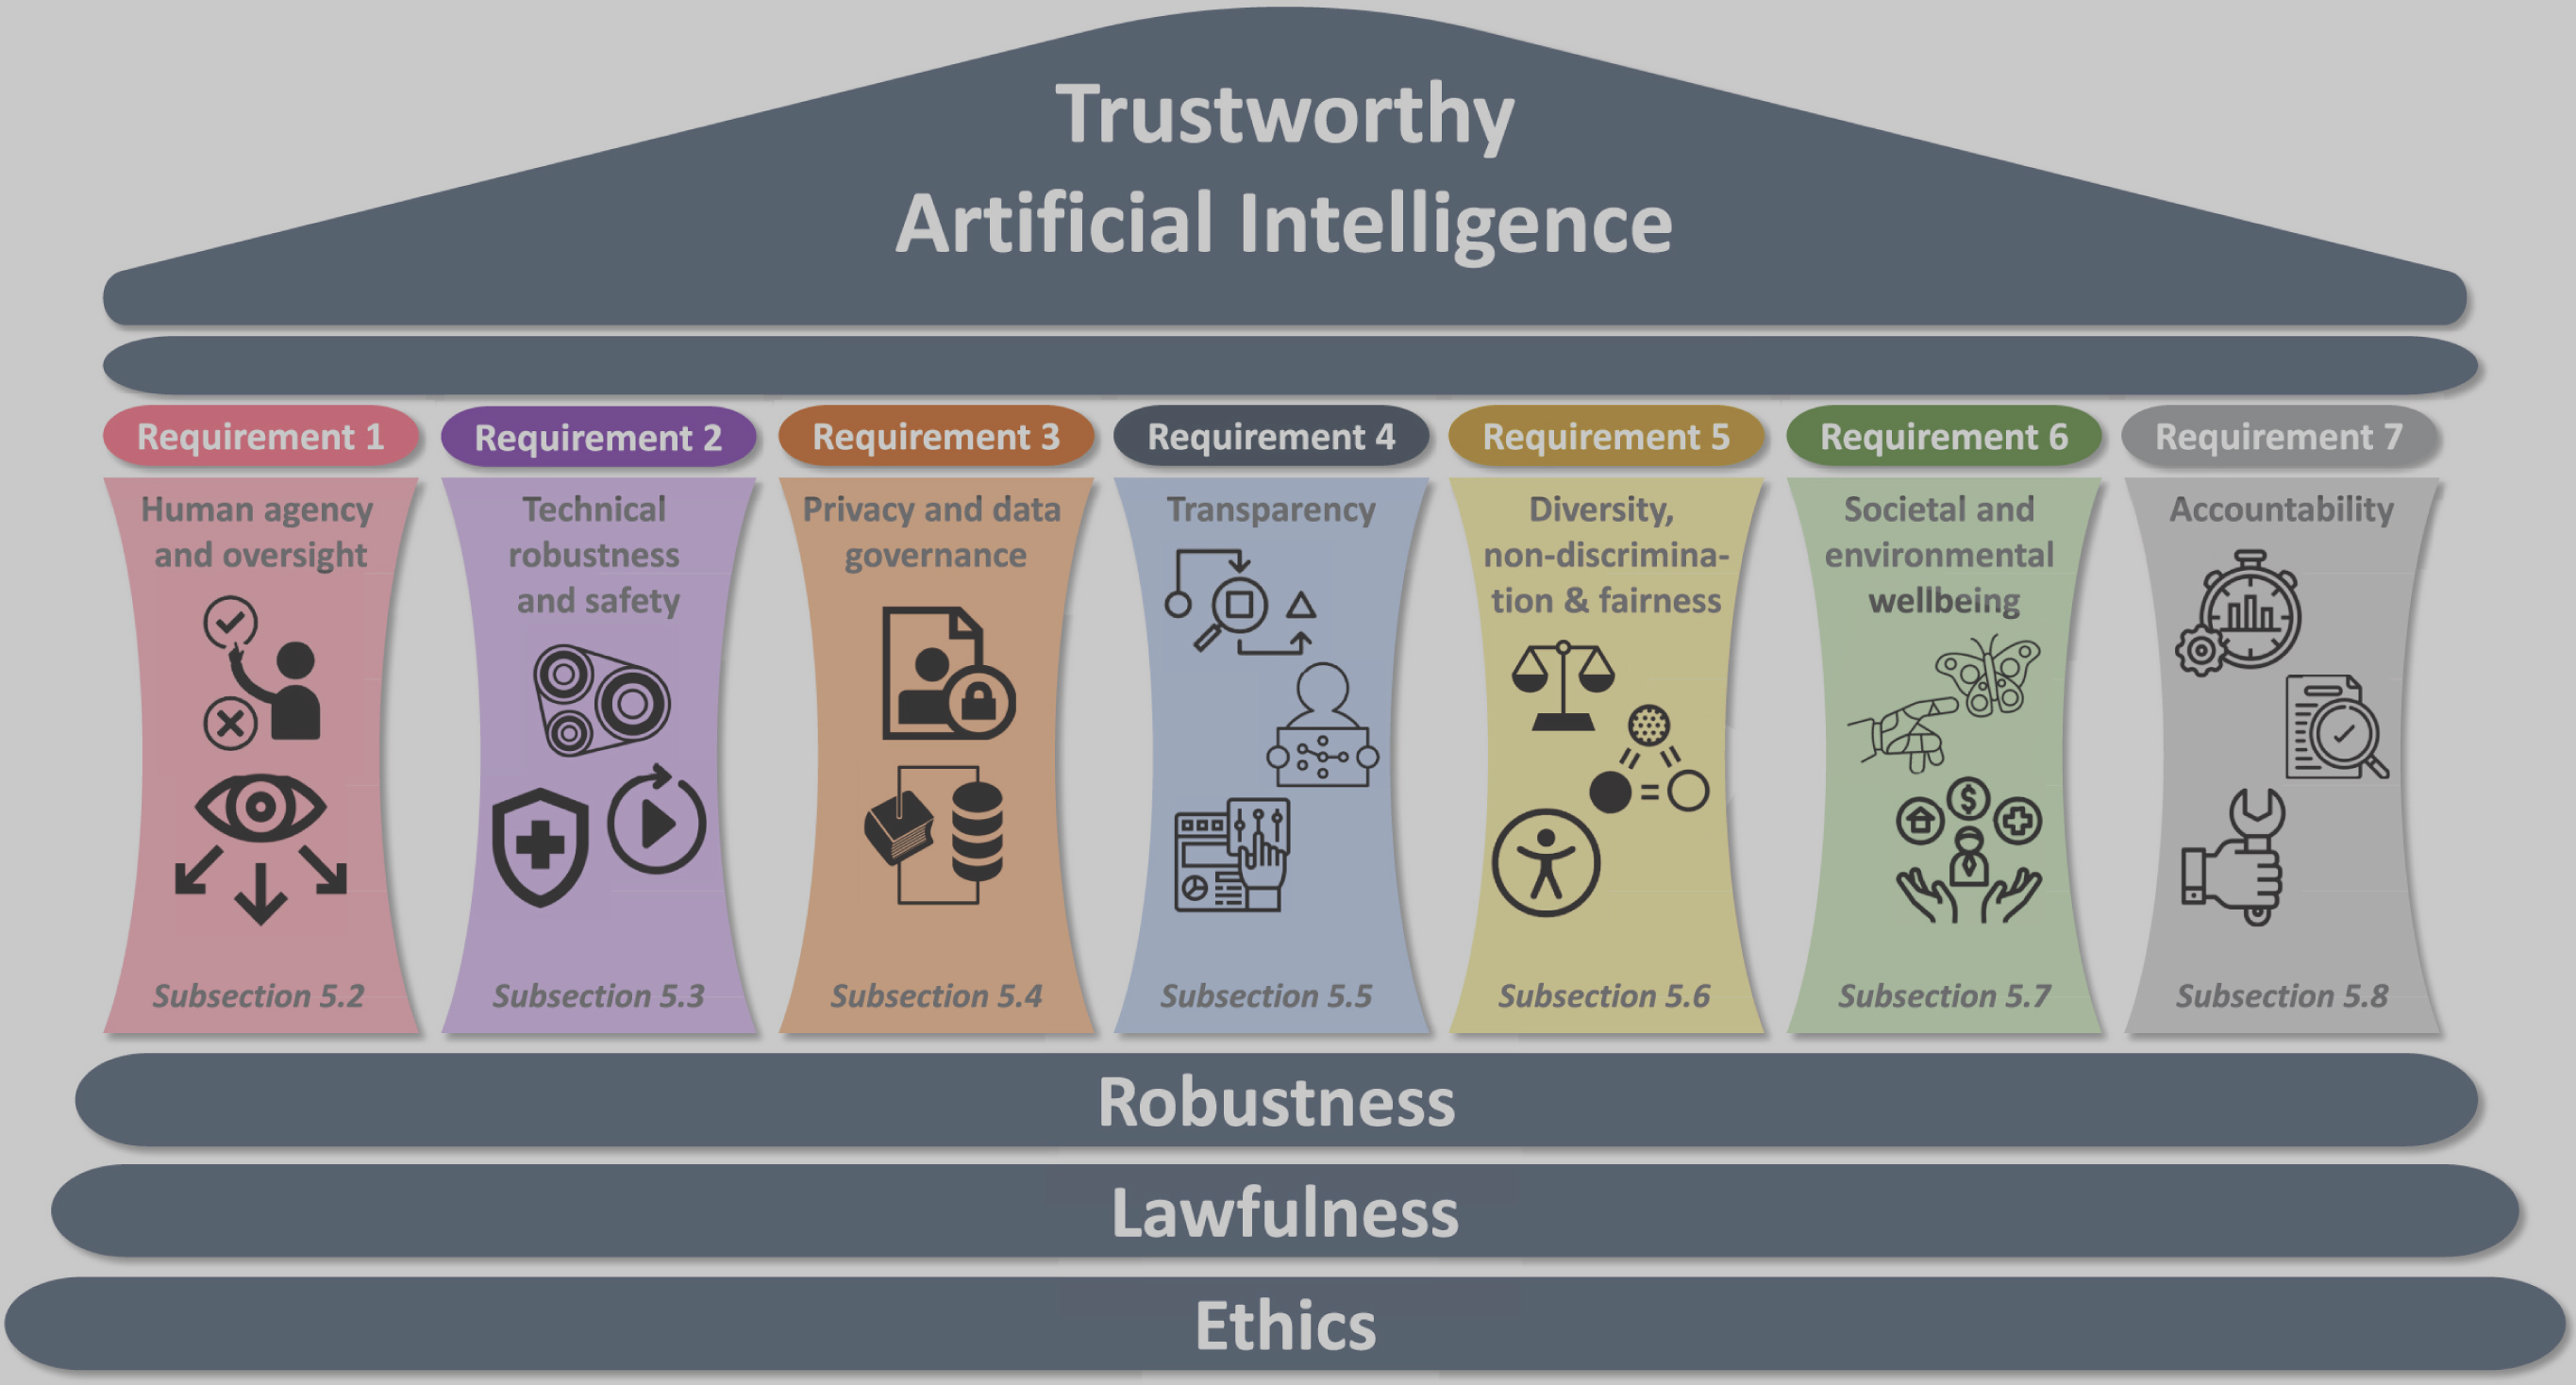
\includegraphics[width=\textwidth]{trustworthy_ai}
  \caption{Image credit \href{https://montrealethics.ai/}{Montreal AI Ethics Institute}}
  \label{fig:trustworthy-ai}
\end{figure}

\section{Large Language Model: Threat-Informed Defense}

The purpose of the checklist is to help organizations understand the risks and
benefits of using LLM by focusing on LLM threats that come from released models
or services from third-party models. It will also include and improve existing
resilience defensive techniques. Open source resources from both MITRE Engenuity
and OWASP are referenced.

\clearpage

\begin{figure}[h]
  \centering
  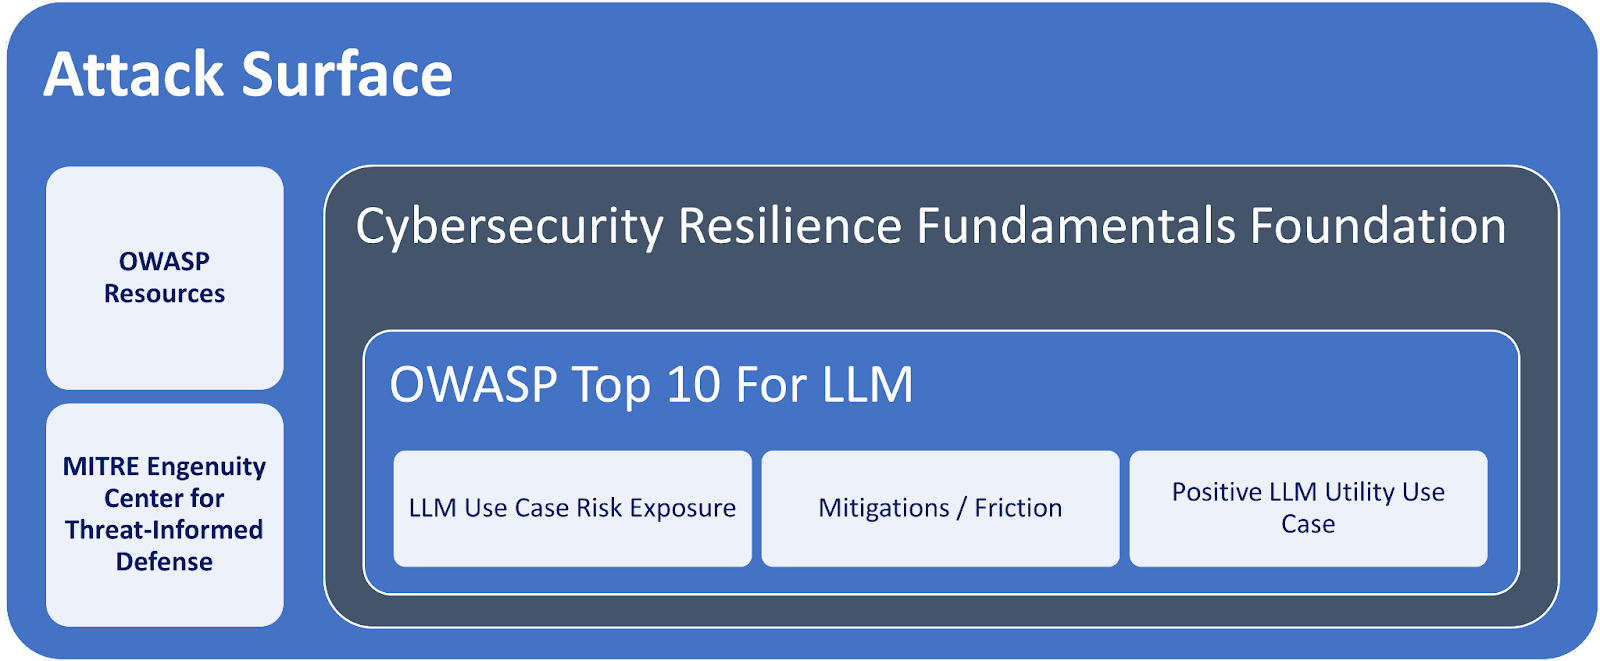
\includegraphics[width=\textwidth]{llm_attack_surface}
  \caption{Image of integrating LLM Security with OWASP and MITRE resources}
  \label{fig:llm-attack-surface}
\end{figure}

\section{Why a Checklist?}

Checklists can help with strategy development by ensuring thoroughness,
clarifying goals, fostering consistency, and allowing for focused, deliberate
effort, all of which may result in fewer oversights. Following the list can
build confidence in a path to secure adoption while sparking ideas for future
business cases moving forward. It\'s a very forward and very practical way to
achieve continuous improvement.

\section{Not Comprehensive}

This document is intended to support organizations in developing an initial LLM
strategy in a rapidly changing technical, legal, and regulatory environment.
Organizations should extend assessments and practices beyond the scope of the
provided checklist.
